\documentclass[sigplan,review,anonymous]{acmart}

% EuroSys 2027 review configuration.  Compile with TEXINPUTS/BSTINPUTS as
% documented in README.md so that the downloaded ACM template is used.
\setcopyright{none}
\settopmatter{printfolios=true,printacmref=false,printccs=false}
\renewcommand\footnotetextcopyrightpermission[1]{}
\pagestyle{plain}
\raggedbottom
\acmConference[EuroSys '27]{European Conference on Computer Systems}%
  {April 19--23, 2027}{Rabat, Morocco}
\acmYear{2027}
\copyrightyear{2027}
\acmDOI{}
\acmISBN{}
\acmSubmissionID{ANON-000}

\usepackage{amsmath}
\usepackage{array}
\usepackage{booktabs}
\usepackage{float}
\usepackage{graphicx}
\usepackage{xcolor}
\usepackage{url}
% EuroSys requires at least 10 pt text on 12 pt leading, including references.
% acmart inherits an 8 pt bibliography from amsart, so restore the body size.
\renewcommand{\bibliofont}{\normalsize}
% The project-local TinyTeX tree may not have user font maps configured.  Keep
% microtype protrusion but disable font expansion so the draft is reproducible
% without mutating the system TeX installation.
\microtypesetup{expansion=false}
\setlength{\emergencystretch}{1.5em}

\newcommand{\system}{\textsc{AegisKV}}
\newcommand{\HBM}{\textsc{HBM}}
\newcommand{\DRAM}{\textsc{DRAM}}
\newcommand{\SSD}{\textsc{SSD}}

% A compact, dependency-free pseudocode float for the two controller algorithms.
\floatstyle{ruled}
\newfloat{algorithm}{tbp}{loa}
\floatname{algorithm}{Algorithm}

\begin{document}

\title{AegisKV: Slack-Aware KV Management for Fault-Tolerant Agentic LLM Serving}

\author{Anonymous Author(s)}
\affiliation{%
  \institution{Anonymous Institution}
  \country{Anonymous}%
}

\begin{CCSXML}
<ccs2012>
 <concept>
  <concept_id>10010520.10010575.10010755</concept_id>
  <concept_desc>Computer systems organization~Reliability</concept_desc>
  <concept_significance>500</concept_significance>
 </concept>
 <concept>
  <concept_id>10011007.10010940.10010971</concept_id>
  <concept_desc>Software and its engineering~Software fault tolerance</concept_desc>
  <concept_significance>300</concept_significance>
 </concept>
</ccs2012>
\end{CCSXML}
\ccsdesc[500]{Computer systems organization~Reliability}
\ccsdesc[300]{Software and its engineering~Software fault tolerance}
\keywords{large language model serving, KV cache, fault tolerance,
agentic workflow, recovery}

\begin{abstract}
Agentic applications turn one user task into a dependency graph of long,
multi-turn model requests.  A GPU failure can discard a large amount of live
key--value (KV) state, yet protecting every byte in the fastest tier imposes
substantial memory and transfer cost on healthy serving.  More importantly,
equal-sized KV prefixes need not have equal recovery value: a delay on a
workflow-critical branch extends completion time, whereas a parallel branch
may absorb the same delay.  We present \system{}, which uses workflow Slack to
connect normal-period KV management with failure-time recovery.  At request and
tool boundaries, the application predicts remaining agent durations with GBDT
and computes branch Slack with CPM.  The serving control plane converts the
result into the reduction in Slack-exposed recovery delay.  Its
\textsc{SlackLandlord} policy uses this value to admit and evict variable-size,
continuous KV chunks in DRAM and optional peer HBM, while
\textsc{GuardedAIMD} adapts only the peer-HBM capacity envelope to foreground
memory pressure.  On failure, the same remaining Slack orders adoption,
loading, and recomputation on a compatible target.  Complete-chunk commit,
version checks, and output fencing preserve correctness when copies or workers
fail.  The design handles one fail-stop serving domain at a time and builds on
existing KV storage and transfer paths.
% Add one quantitative outcome sentence here only after the paired physical
% evaluation has a frozen configuration, sample count, and confidence interval.
\end{abstract}

\maketitle

\section{Introduction}
\label{sec:introduction}

LLM serving systems increasingly execute \emph{workflows}, not isolated
requests.  An agent may invoke several model replicas and tools in parallel,
join their outputs, and issue another round of long-context requests.  The KV
cache accumulated along this execution is expensive to regenerate.  When a
worker fails, restarting from tokens can delay not only the interrupted request
but every downstream node waiting for it.

Existing systems reduce this cost by streaming, checkpointing, or offloading KV
state to peer GPUs, host memory, or storage
~\cite{strati2024dejavu,jayakody2026ghostserve,qin2025mooncake,xie2025hicache}.
These mechanisms answer how to move and restore KV efficiently.  They do not,
by themselves, determine which live KV state most reduces a workflow's
failure-induced completion delay when capacity is scarce.  Normal cache signals
such as size, recency, and expected reuse are insufficient: two equal-sized
requests can sit on different parallel branches, so the same recovery pause can
be exposed on one branch and hidden behind useful work on the other.

The key observation is simple.  A branch's remaining \emph{Slack} is the delay
it can absorb before it extends the next mandatory join.  If a failure adds less
than that Slack, faster recovery does not change workflow completion time; once
the pause exceeds Slack, each additional second is user visible.  Slack thus
provides a request-level value that the application can compute from workflow
dependencies but the KV manager cannot infer locally.  It also evolves after
every request or tool result, so treating an agent as permanently critical is
too coarse.

\system{} applies this observation twice.  At each request or tool boundary,
the application predicts the remaining duration of the causally visible agent
branches and runs CPM to update their Slack.  The next model request carries
one scalar.  During normal operation, the Controller compares the reduction in
Slack-exposed recovery delay from protecting a complete KV chunk with the harm
of evicting resident chunks.  During recovery, it uses the same updated Slack
to order peer-HBM adoption, DRAM loading, and recomputation.  This shared signal
keeps protection and recovery aligned: state protected because it is urgent is
also recovered early if the failure occurs.

Turning the observation into an online system raises two practical problems.
First, Slack changes much more frequently than large KV regions should move.
\textsc{SlackLandlord} therefore changes request-level credit lazily and moves
data only on chunk sealing or capacity pressure.  A per-pool heap exposes one
prefix-safe eviction tail per request, avoiding a global re-sort of all pages.
Second, peer-HBM protection must never endanger
foreground allocation.  \textsc{GuardedAIMD} adjusts a target's shadow-HBM
quota on a slow time scale, while the Worker allocator remains the final
capacity authority.  DRAM and SSD continue to use the underlying Store and
transfer machinery.

\system{} deliberately makes a narrow fault-tolerance claim.  It handles one
fail-stop serving domain at a time, recovers a request on a Router-selected
target with the same model and parallel layout, and uses only complete,
version-compatible KV chunks.  Missing or stale metadata falls back to
recomputation.  Slack affects performance priority, never correctness or
physical capacity.

This paper makes three contributions:

\begin{itemize}
  \item It identifies workflow Slack as the missing value signal for KV fault
  tolerance and quantifies, using a public agent trace, why parallel branches
  expose different failure costs (\S\ref{sec:background}).

  \item It designs \system{}, whose \textsc{SlackLandlord} policy converts the
  same fail-now recovery model into normal-period admission and eviction
  credits and failure-time recovery order.  The policy manages variable-size,
  continuous KV prefixes without solving an online MCF or MILP
  (\S\ref{sec:design}).

  \item It separates policy from safety: \textsc{GuardedAIMD} adapts only the
  peer-HBM envelope, Workers enforce local capacity, and the commit and fencing
  protocol prevents partial KV or duplicate output from becoming visible
  (\S\ref{sec:control-plane}--\S\ref{sec:end-to-end}).
\end{itemize}

% Evaluation contribution and headline numbers belong here only after the
% physical implementation and paired experiment gates in Section 5 pass.

\section{Background and Motivation}
\label{sec:background}

% 中文导读（仅供写作与审阅，不进入最终 PDF）：
% 本节按照“故障恢复为什么变贵 -> 为什么不同请求的恢复价值不同 -> 为什么现有 KV 管理缺少必要信息”展开。
% 1. agentic workflow -> retry 需要重算的前缀通常越长，因此长上下文放大恢复代价。
% 2. Workflow Completion Time（WCT）， Slack。
% 3. 现有推理引擎主要依据 KV 大小、位置、复用和系统负载管理缓存，却缺少 workflow 依赖与 Slack；
% 因此 KV Priority 应由上层 agentic 信息决定，并表示为一个 chunk 对 failure-induced WCT 的边际降低。

% 本节主文只保留一组 Motivation 图像：
% Figure~\ref{fig:real-cc-parallel}：三个子图使用同一 Real CC trace；依次给出严格并行
%    subagent 秒差 CDF、可编辑 Draw.io workflow 实例、以及 failure-position counterfactual。
% figures/motivation-recovery-scaling.pdf 与
% figures/motivation-kv-publication-comparison.pdf 移入 appendix/implementation audit；
% 未校准 component model 不占用主文 Motivation 空间。

\subsection{Agentic context growth amplifies GPU-failure recovery cost}

An agentic application is a DAG of model and tool calls whose later requests
consume an accumulated transcript.  Prefix caching can reuse prior KV, but
each tool return still starts a new admission/prefill/decode lifecycle
~\cite{abhyankar2024infercept}.  Context and KV therefore tend to grow across
turns.  A worker failure discards this execution state; a compatible prefix can
avoid re-prefill, while an absent suffix must be recomputed.

Already generated KV is immutable under a fixed model and token sequence, so
the runtime seals it in groups of $G$ tokens.  Only a complete contiguous
prefix is a recovery point.  Decisions are online: future groups and final
length are unknown; per-request checkpoints are coarse, whereas independent
chunk rewards double-count overlapping prefixes.  \system{} instead values
prefix-bundle actions whose recovery plan may combine peer HBM, Store reads,
and recomputation.  Service bounds include setup, contention, adoption, and
resume rather than hardware peak bandwidth.  Protection consumes HBM, Store
quota, and transfer capacity also needed by healthy traffic, so the objective
must price workflow benefit without imposing a normal-path tax.  Evaluation
separates component bounds from physical failure-to-ready time.

\subsection{Workflow completion exposes critical requests}

The user-visible unit is workflow completion time
$\mathrm{WCT}_w=C_w-A_w$.  We measure fault-added
$[\mathrm{WCT}^{\mathrm{fail}}_w-\mathrm{WCT}^{\mathrm{nf}}_w]_+$ against a
paired no-failure run, so changing the healthy schedule cannot masquerade as
recovery benefit.  A request matters only through delay propagated to the
terminal: one branch can block a fan-in while another absorbs the same pause.

Figure~\ref{fig:real-cc-parallel} quantifies this structure in the public Real
CC trace~\cite{semianalysis2026cctraces}.  A parser fan-out is a maximal
consecutive run of top-level subagent records with at least two branches; we
retain it only when all recorded branch intervals share a nonempty common
overlap.  For fan-out $g$, let
$R_g=\max_{a\in g}d_a-\min_{a\in g}d_a$.  Each workflow contributes one CDF
sample, $R_w=\max_{g\in G_w}R_g$, so workflows with many fan-outs are not
overweighted and branches from different episodes are never compared.  Of 393
workflows, 124 contain 292 retained fan-outs and 944 branch executions.  The
median $R_w$ is 140.611~s and the 90th percentile is 1570.290~s.

Panels~(b,c) use workflow 8ab0a089\ldots: five branches last 110.3, 116.7,
78.9, 117.9, and 107.1~s (39.0~s gap).  Because the trace has no parent ID, we
reconstruct its isolated fan-out/fan-in from top-level order and timestamps.
At common active time $t_f=349.5$~s, panel~(c) combines each real 65--112K
prefix and observed fan-in slack with the Qwen3-235B-A22B
TP8$\times$PP4$\times$EP8 AIConfigurator recomputation model.  Exposed delays
are 0, 17.2, 0, 35.9, and 21.4~s.  This trace-plus-model counterfactual is not a
Claude measurement or paired failure run.

\begin{figure*}[t]
  \centering
  \begin{minipage}[b]{0.285\textwidth}
    \centering
    \parbox[c][1.72in][c]{\linewidth}{\centering
      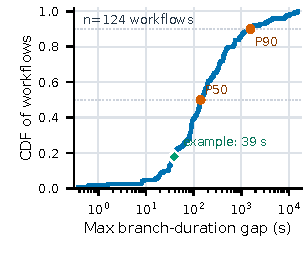
\includegraphics[width=\linewidth]{figures/real-cc-parallel-subagent-duration.pdf}}
    \small (a) Parallel-runtime gap.
  \end{minipage}\hfill
  \begin{minipage}[b]{0.39\textwidth}
    \centering
    \parbox[c][1.72in][c]{\linewidth}{\centering
      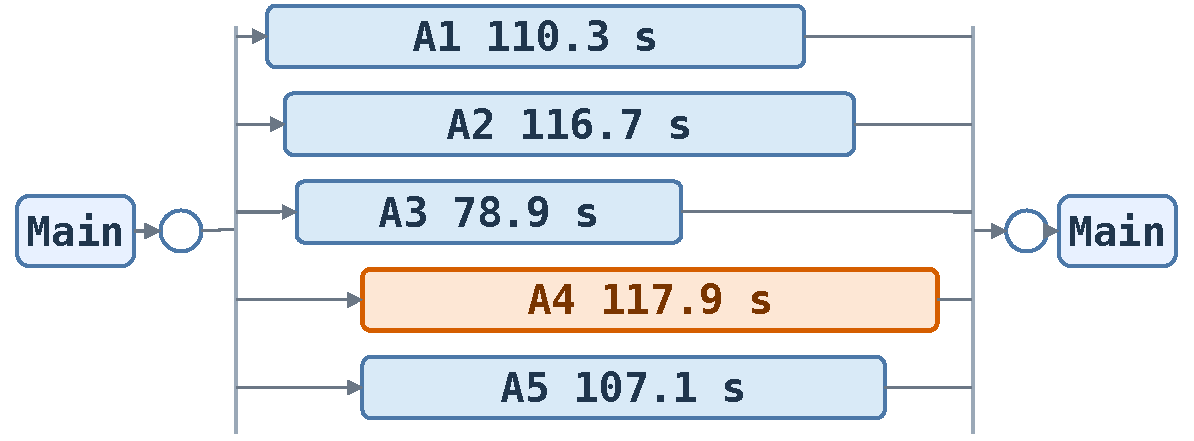
\includegraphics[width=\linewidth]{figures/real-cc-workflow-8ab0a089.pdf}}
    \small (b) Real CC workflow example.
  \end{minipage}\hfill
  \begin{minipage}[b]{0.285\textwidth}
    \centering
    \parbox[c][1.72in][c]{\linewidth}{\centering
      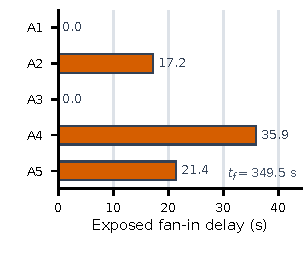
\includegraphics[width=\linewidth]{figures/real-cc-failure-position-counterfactual.pdf}}
    \small (c) Failure-position sensitivity.
  \end{minipage}
  \caption{Parallel execution and failure-position sensitivity in the Real CC
  trace.  Panel~(a) reports the CDF of each eligible workflow's largest
  within-fan-out slowest-minus-fastest duration gap.  Panel~(b) reconstructs a
  selected five-way fan-out from workflow 8ab0a089\ldots, whose
  slowest--fastest gap is 39.0~s.  Panel~(c) marks all five failure targets and
  subtracts each branch's observed fan-in slack from its configuration-predicted
  prefix-recomputation time at $t_f=349.5$~s.  Panels~(a) and~(b) summarize trace
  observations; panel~(c) is a trace-plus-AIConfigurator counterfactual rather
  than an end-to-end measurement.}
  \Description{Three panels show a Real CC workflow-level duration-gap CDF, a
  compact five-way fan-out with a 39-second branch-duration gap, and a
  horizontal-bar counterfactual for all five failure targets.}
  \label{fig:real-cc-parallel}
\end{figure*}

At each LLM-request or tool-call completion, Algorithm~1 uses a GBDT model to
predict the remaining duration $\widehat T_r(t)$ of each active branch and CPM
to identify its next mandatory fan-in.  The unknown suffix shared after that
join cancels from the comparison, so the application need not predict the
entire future workflow.  For branch $r$, it computes
\begin{equation}
  s_r(t)=\left[\max_{j\ne r}\widehat T_j(t)-\widehat T_r(t)\right]_+.
  \label{eq:slack}
\end{equation}
The next request carries this Slack as ordinary metadata.  The serving layer
decreases it by elapsed request time, and the next application response
replaces it with a new GBDT/CPM estimate.  Slack is therefore dynamic rather
than an agent label or operator SLO.  Prediction error may change protection
priority, but it cannot bypass physical resource limits or make an incomplete
KV group recoverable.

\subsection{KV priority must incorporate agentic information}

Local size, tier, recency, reuse, and load signals cannot reveal whether a
pause blocks a workflow join.  The missing input is the marginal reduction in
failure-induced WCT produced by a complete KV action, after Slack and
tier-specific resource cost.  Agentic information augments rather than replaces
the engine's placement signals.

\paragraph{Serving and workflow substrates.}
PagedAttention and SGLang provide efficient page/prefix management
~\cite{kwon2023vllm,zheng2024sglang}; Mooncake, HiCache, SYMPHONY, Strata, and
Bidaw provide disaggregated or hierarchical KV placement and loading
~\cite{qin2025mooncake,xie2025hicache,agarwal2026symphony,
xie2026strata,hu2026bidaw}.  Parrot, KVFlow, Pythia, and Agentix expose
workflow structure or predictability to serving
~\cite{lin2024parrot,pan2025kvflow,yu2026pythia,luo2026agentix}.
These are substrates, not limitations: \system{} claims neither tiering nor
DAG analysis.  Their cache state, reuse, and load signals do not alone encode
how a worker-failure pause propagates to workflow completion.

\paragraph{Agent-aware and physical KV scheduling.}
TokenCake, Continuum, PBKV, and TokenDance already use graph criticality,
waiting time, future invocation, or synchronized rounds for normal-time KV
management~\cite{bian2026tokencake,li2026continuum,
zheng2026pbkv,bian2026tokendance}.  CacheFlow overlaps recomputation and I/O
across tokens, layers, and GPUs and schedules batch restoration
~\cite{nian2026cacheflow}.  We therefore claim neither the first agent-aware
KV manager nor hybrid/parallel restoration.  A CacheFlow-like engine can
implement the restore/load/recompute path; our distinct input is workflow
Slack used both before and after a worker failure.

Configured MooncakeStoreConnector and HiCache paths may expose only a committed
prefix at a decode-time failure; the live tail still requires recomputation.
Their exact publication point depends on connector and write policy, so the
configuration-specific timeline is deferred to the appendix.  Cache presence
alone is not a crash-consistent resume contract.

\paragraph{Recovery and workflow Slack.}
D\'ej\`aVu streams KV for recovery; GhostServe, RaidServe, KevlarFlow, LUMEN,
and Concordia provide shadow/checkpoint, routing, or execution-state recovery
mechanisms~\cite{strati2024dejavu,jayakody2026ghostserve,xu2026raidserve,
qian2026kevlarflow,cao2026lumen,gan2026concordia}.  MFS schedules normal
multi-stage flows by laxity and TENT supplies deadline-aware resilient data
movement~\cite{sun2026mfs,ren2026tent}.  Thus checkpointing, load-aware
recovery, deadline fields, and flow scheduling are not our novelty.  Our
narrow claim is the coupling: the same workflow Slack values Store/peer
protection before a worker fail-stop and orders the joint
restore/load/recompute path afterward under serving-resource limits.

Classic real-time systems already use task slack to place checkpoints and
reserve rollback work, including distributed DAG tasks scheduled by EDF
~\cite{melhem2004interplay,acharya2008dynamic}.  Hence neither ``slack-aware
checkpointing'' nor Slack-ordered recovery is our novelty.  Our narrower claim
is its KV realization: compute Slack from an evolving agent workflow, use it to
value Store or peer-HBM state before fail-stop, and reuse it to order recovery
afterward.

% The archived preliminary SGLSim figure is intentionally excluded: it does
% not implement the final policy or physical recovery path.  Paper claims will
% use the final paired evaluation rather than promote that diagnostic.

\subsection{Design requirements and scope}

The design must therefore optimize workflow-visible delay over complete KV
groups, admit only failure-valid shards, isolate healthy traffic, and keep
analytical, protocol, and empirical evidence distinct.

We consider one declared fail-stop serving domain at a time and label
process/GPU and host failures separately; colocated state is lost.  The Router,
failure-isolated request log, Store quorum, network, and a model-loaded
same-layout target survive.  The Router---not \textsc{SlackLandlord}---selects that target,
which resumes from a surviving continuous prefix or recomputes.  We do not
splice pipeline stages.  Correlated/Store/Router failures, corrupted weights,
Byzantine faults, and cross-layout recovery are outside the first claim.

% Synchronized from AegisKV/design/current_design.md.
% current_design.md is the source of truth; update it before editing this file.
% Source-SHA256: 915886a3fbca8270eb55c1e5867f4c01bff1b0edaa48ab0294972a3392a20682
\section{System Design}
\label{sec:design}

\subsection{Overview}

\system{} has three layers (Figure~\ref{fig:system-overview}).  The application
runtime predicts agent duration and computes Slack.  The serving control plane
contains the Router and Aegis Controller: the Router owns route and output
state, while the Controller incorporates Store Master and owns KV metadata,
protection, recovery order, and protection budgets.  Workers execute inference,
KV movement, and recovery under locally enforced limits.

\begin{figure*}[t]
  \centering
  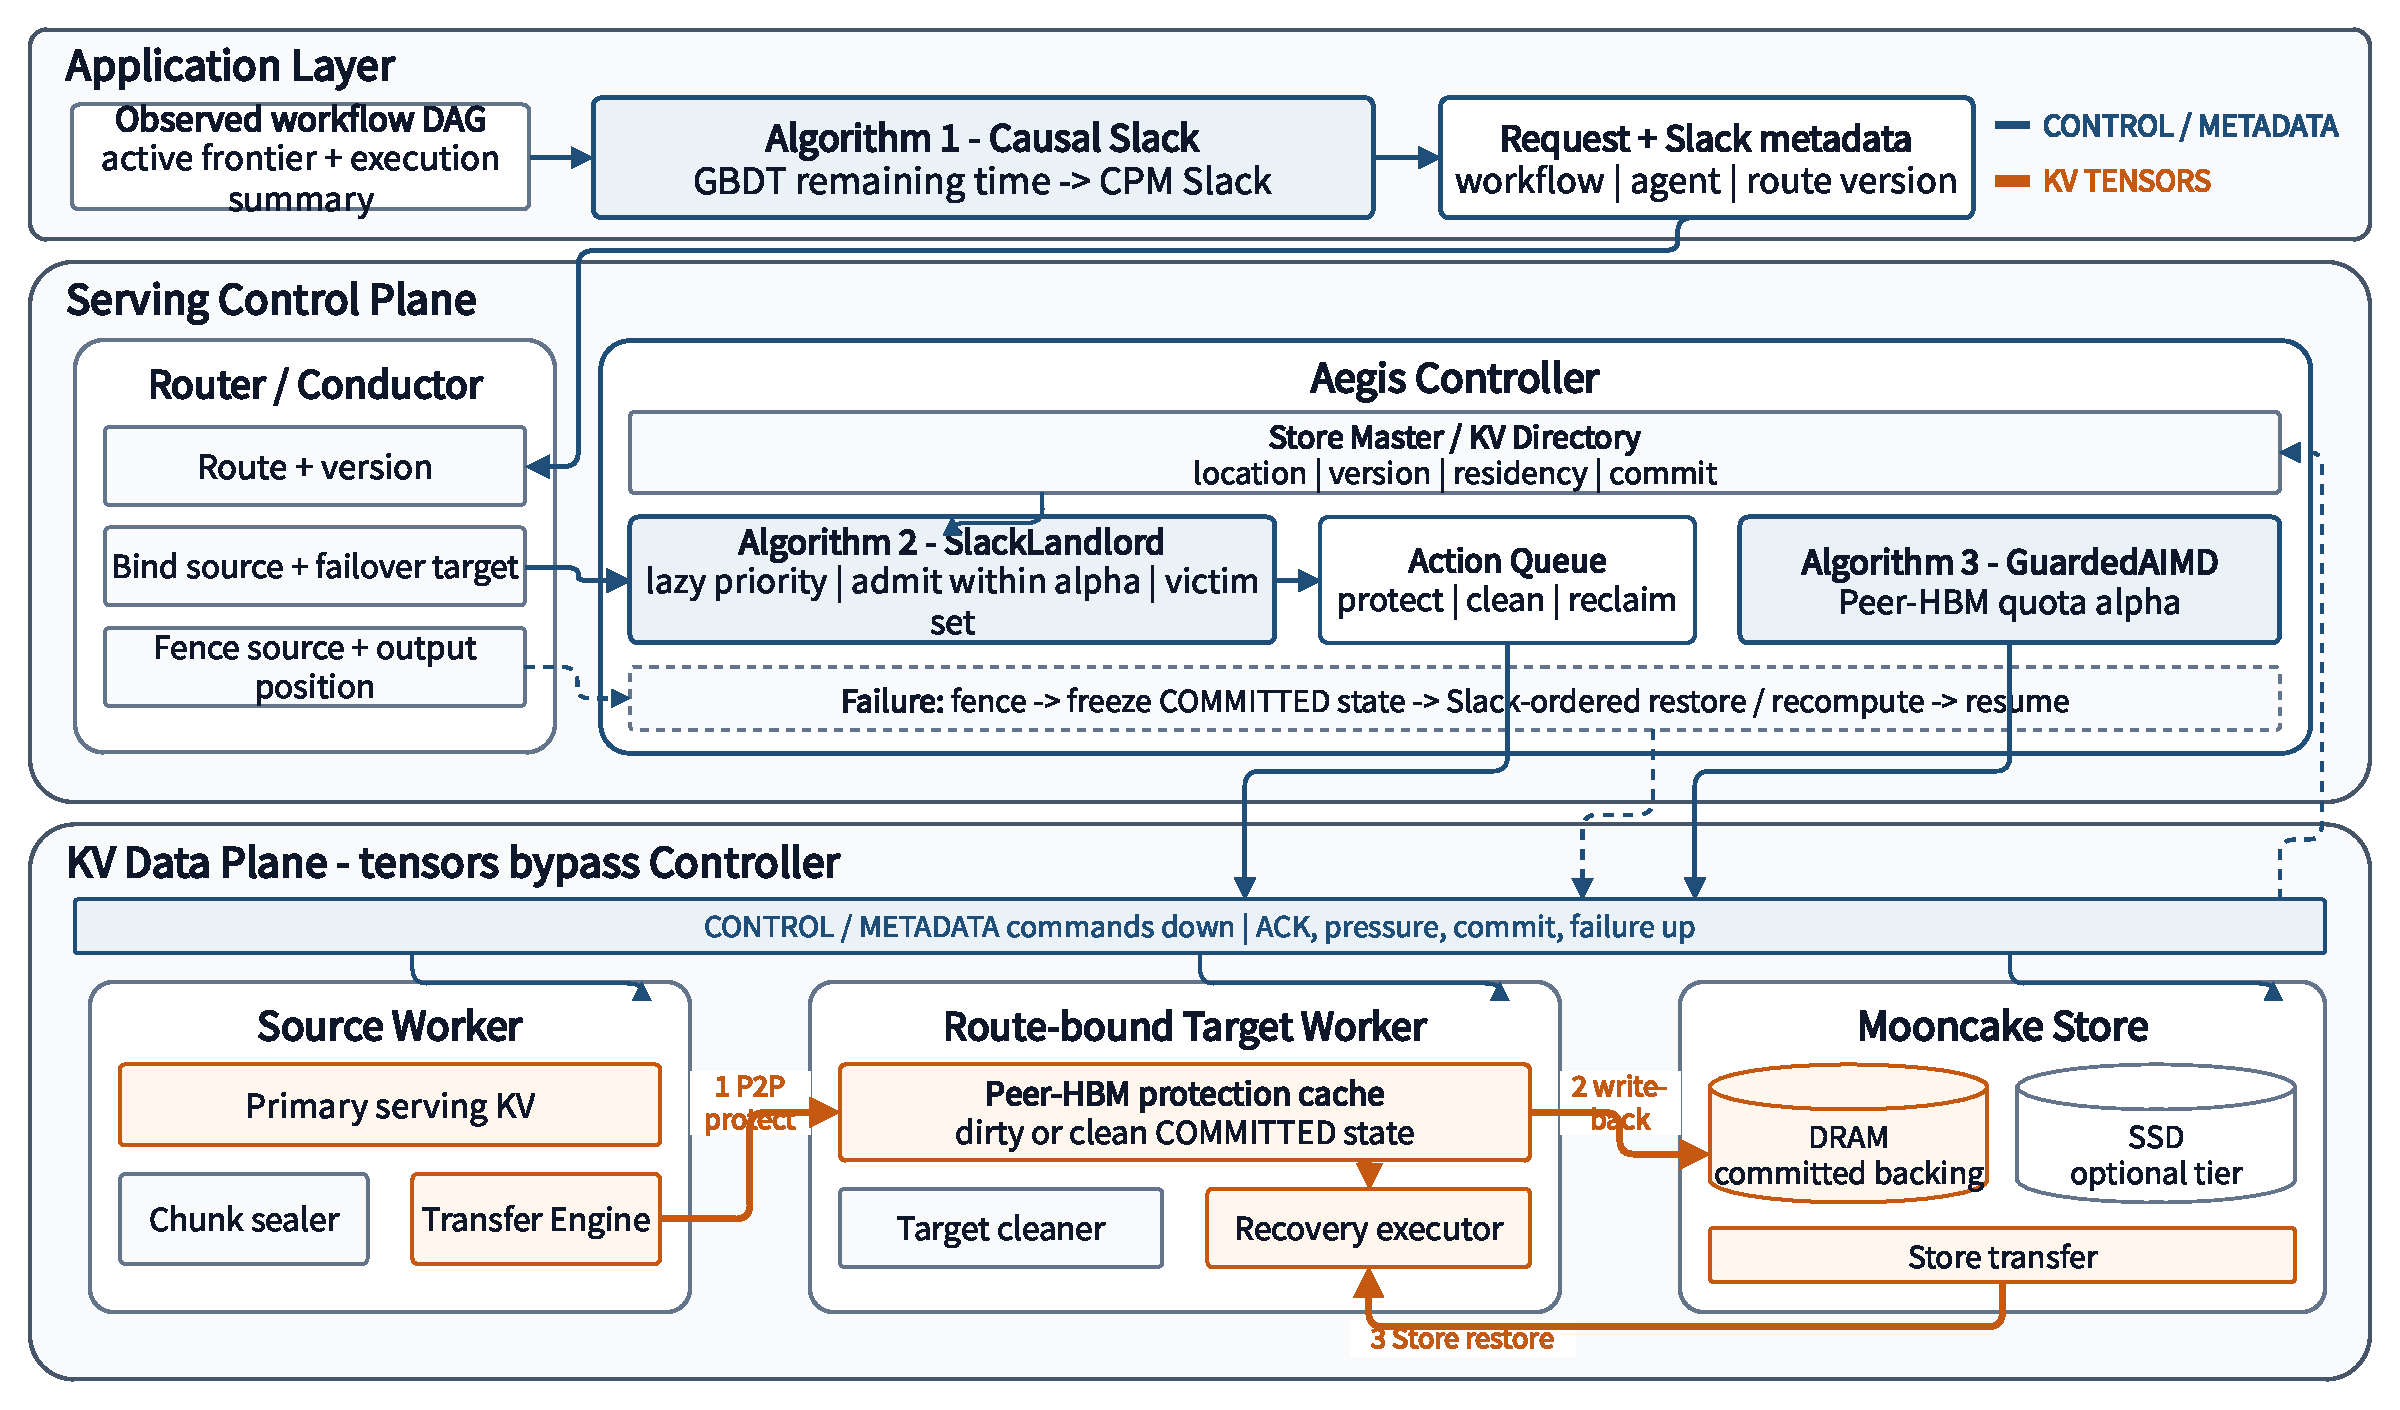
\includegraphics[width=0.89\textwidth]{figures/system-overview.pdf}
  \caption{\system{} overview.  One workflow Slack signal drives normal-period
  protection and failure-time recovery.  Blue arrows carry control and
  metadata; orange arrows carry KV tensors directly among Workers and Store.}
  \Description{A three-layer architecture.  The application layer converts an
  observed workflow DAG into causal Slack metadata.  The serving control plane
  contains the Router, KV Directory, SlackLandlord, action queue, and
  GuardedAIMD.  In the KV data plane, orange paths protect source KV in a
  route-bound target Worker's peer-HBM cache, write committed data back to
  Store DRAM, and restore it to the target after failure; blue paths carry
  commands and acknowledgements.}
  \label{fig:system-overview}
\end{figure*}

Only the application observes agent dependencies, so it computes Slack.  The
Controller has the failure-domain and KV-location view needed by
\textsc{SlackLandlord} and \textsc{GuardedAIMD}; Workers make no global
placement decision.  Persistent \emph{KV Directory} state (chunk locations,
versions, occupancy, and commits) is separated from reconstructible policy
state (pool rent, credit heaps, queues, and control-window counters).

The normal path is short.  A Worker seals a complete KV chunk; the Controller
forms a DRAM candidate or uses the Router-fixed Peer-HBM target; and
\textsc{SlackLandlord} selects bypass or an eviction set from the target's
currently exposed free bytes.  The Controller then evicts that set, allocates
the final space, and records the new chunk as \textsc{Pending}; the action queue
then starts a direct asynchronous copy.  The directory changes it to
\textsc{Committed} only after every shard acknowledges and its version remains
valid.  A failed copy becomes \textsc{Aborted} and releases its space; evicted
replicas are not restored.  On
failure, the Router fences the source and activates a
route-bound target.  The Controller then freezes committed state, chooses
Peer-HBM, DRAM, or recomputation per ready request, and orders recovery with
the same Slack.  KV bytes never pass through the Controller.

\subsection{Application layer: GBDT and CPM}
\label{sec:application-layer}

At each LLM-request or tool-call completion, the workflow runtime uses GBDT to
predict remaining agent durations and runs CPM on the causally revealed
residual DAG from the active frontier to the next join.  If $ES_i$ and $LS_i$
are branch $i$'s earliest and latest starts, the application computes
\begin{equation}
  s_i=[LS_i-ES_i]^+.
  \label{eq:design-slack}
\end{equation}
For one fan-out/join, this reduces to
$[\max_j\widehat T_j-\widehat T_i]^+$.
In Algorithm~\ref{alg:slack-update}, $\mathcal N_t$ is the set of visible
agent nodes, $\mathcal A_t$ is the active frontier, and
$\mathcal V_t^{\mathrm{start}}$ and $\mathcal V_t^{\mathrm{end}}$ are the
start and end nodes.  An active node uses predicted remaining duration, a visible
not-yet-started node uses predicted full duration, and a structural node has
zero weight.
It attaches $s_i$ to the next request as ordinary metadata.  The Controller
decreases it by elapsed request time, and the next application update replaces
the old value.  Missing Slack, an incomplete residual sub-DAG, or a missing
node prediction yields zero Slack.  Prediction error changes priority but
cannot violate resource or recovery safety.

Algorithm~\ref{alg:slack-update} shows the complete online path.  On each
request or tool return, \textsc{UpdateSlack} records the event (line 1), orders
the residual DAG and identifies its start and end nodes (line 2), then predicts
visible node weights in an explicit loop (lines 3--5).  The forward loop
computes earliest starts in topological order (lines 6--8).  The end-node
completion span initializes the backward loops, which compute latest starts in
reverse topological order (lines 9--14).  A final loop computes, validates,
stores, and attaches active-branch Slack (lines 15--17).  Repeated returns
therefore revise Slack causally; the algorithm never reads a future output
length, completion time, or failure location.

For fixed $G_t$ and nonnegative predicted weights, the two passes compute exact
CPM total float on that residual DAG.  This is not a guarantee of true future
Slack; incomplete inputs fail closed to zero and later returns revise the estimate.

For $N$ visible agent nodes, $F$ features, $M$ depth-$d$ trees, and residual
DAG $G_t=(V_t,E_t)$, one update costs
$O(N(F+Md)+|V_t|+|E_t|)$ time and $O(|V_t|+|E_t|)$ state excluding the fixed
model.  With a fixed feature schema and model, time is
$O(|V_t|+|E_t|)$ and is paid only on a request or tool return, not per token.

% Compiled by sections/03-system-design-v2.tex.
% Design-SHA256: 915886a3fbca8270eb55c1e5867f4c01bff1b0edaa48ab0294972a3392a20682
\begin{algorithm}[t]
\caption{Online GBDT--CPM Slack update}
\label{alg:slack-update}
\begin{tabular}{@{}r@{\hspace{0.5em}}>{\raggedright\arraybackslash}p{\dimexpr\columnwidth-2.5em\relax}@{}}
\multicolumn{2}{@{}>{\raggedright\arraybackslash}p{\columnwidth}@{}}{\textbf{UpdateSlack}$(e,t)$}\\
\multicolumn{2}{@{}>{\raggedright\arraybackslash}p{\columnwidth}@{}}{\textit{Symbols.} $G_t=(V_t,E_t)$: residual DAG; $H_t$: execution summary; $\mathcal N_t/\mathcal A_t$: agent nodes/active frontier; $\mathcal V_t^{\mathrm{start}}/\mathcal V_t^{\mathrm{end}}$: start/end-node sets.}\\
\multicolumn{2}{@{}>{\raggedright\arraybackslash}p{\columnwidth}@{}}{$f_\theta/\phi_v$: GBDT/features; $\hat w_v$: predicted time; $ES_v/LS_v$: earliest/latest start; $\sigma_i=(s_i,t)$; $\operatorname{Valid}_i$: complete causal input.}\\
1 & $(G_t=(V_t,E_t),H_t,\mathcal N_t,\mathcal A_t)\gets\operatorname{Observe}(G_{t^-},H_{t^-},e)$.\\
2 & $\pi\gets\operatorname{Topo}(G_t)$; $\mathcal V_t^{\mathrm{start}}\gets\{v:\operatorname{pred}(v)=\varnothing\}$; $\mathcal V_t^{\mathrm{end}}\gets\{v:\operatorname{succ}(v)=\varnothing\}$.\\
3 & \textbf{for} $v\in V_t$ \textbf{do}\\
4 & $\quad\hat w_v\gets0$; \textbf{if} $v\in\mathcal N_t$ \textbf{then} $\hat w_v\gets f_\theta(\phi_v(G_t,H_t))$.\\
5 & \textbf{end for}\\
6 & \textbf{for} $v\in\pi$ \textbf{do}\\
7 & $\quad$\textbf{if} $v\in\mathcal V_t^{\mathrm{start}}$ \textbf{then} $ES_v\gets0$; \textbf{else} $ES_v\gets\max_{u\in\operatorname{pred}(v)}(ES_u+\hat w_u)$.\\
8 & \textbf{end for}\\
9 & $C_t\gets\max_{v\in\mathcal V_t^{\mathrm{end}}}(ES_v+\hat w_v)$.\\
10 & \textbf{for} $v\in\mathcal V_t^{\mathrm{end}}$ \textbf{do} $LS_v\gets C_t-\hat w_v$.\\
11 & \textbf{end for}\\
12 & \textbf{for} $v\in\operatorname{rev}(\pi)\setminus\mathcal V_t^{\mathrm{end}}$ \textbf{do}\\
13 & $\quad LS_v\gets\min_{u\in\operatorname{succ}(v)}LS_u-\hat w_v$.\\
14 & \textbf{end for}\\
15 & \textbf{for} $i\in\mathcal A_t$ \textbf{do}\\
16 & $\quad s_i\gets[LS_i-ES_i]^+$; $\neg\operatorname{Valid}_i\Rightarrow s_i\gets0$; $\sigma_i\gets(s_i,t)$; $\operatorname{meta}(\operatorname{next}(i))[s]\gets s_i$.\\
17 & \textbf{end for}\\
\end{tabular}
\end{algorithm}


\subsection{Serving control plane}
\label{sec:control-plane}

\subsubsection{Router and Conductor}

The Router tracks request-to-Worker mappings, Worker health, route versions,
and committed output positions.  Each route version binds a model, KV ABI,
parallel layout, and compatible failover target.  Peer-HBM protection is
created only on that target.  On failure, the Router fences the source, freezes
output, and activates the target.  A later target may use failure-domain-safe
DRAM, but cannot use Peer HBM belonging to the failed route.

\subsubsection{Aegis Controller}

The Controller incorporates Store Master.  Its KV Directory tracks each
chunk's source domain, route version, completeness, location, and bytes.
Store Master checks the model, KV ABI, parallel layout, and failure domain and
maps a chunk to logical DRAM.  The Router already fixes each request's
Peer-HBM target.  Algorithm 2 therefore receives an already-targeted placement
instead of enumerating pools.  Each target Worker keeps independent HBM
capacity, rent, and heap state.

\paragraph{SlackLandlord.}
Classic Landlord assigns object credit and evicts the object whose normalized
credit is exhausted first~\cite{young2002online}.  \textsc{SlackLandlord} keeps
this credit/rent mechanism but applies it to variable-size KV chunks in DRAM
and Peer HBM.

\textbf{KV chunks.}
Request KV is divided in token order.  The default prefix chunk is 4096 tokens
and the default decode chunk is 256 tokens:
\begin{equation}
 q_{P}=4096,\qquad q_{D}=256.
 \label{eq:chunk-granularity}
\end{equation}
These are configurable implementation parameters; every capacity check uses
the actual bytes $b_c$, which depend on the realized token count, model, KV
type, and parallel layout.  A sealed chunk contains all TP/PP shards for its
token interval.  An open decode tail is not protected until it reaches its
boundary.  Request $i$ maintains DRAM and Peer-HBM frontiers $f_i^D$ and
$f_i^H$.  Admission advances one frontier; eviction removes its suffix tail.
Peer HBM requires the same chunk in DRAM, and deleting a DRAM tail also deletes
its HBM overlay.  Hence both tiers always hold complete continuous prefixes.

\textbf{Recovery harm and credit.}
For committed state $S_i$, a constant-time estimator compares full
recomputation, DRAM, and Peer-HBM recovery, including the slowest shard,
unprotected suffix, and silent replay.  Its Slack-visible harm is
\begin{equation}
 J_i(S_i,t)=[T_i(S_i)-s_i(t)]^+.
 \label{eq:recovery-harm}
\end{equation}
Candidate $x=(c,r)$ targets either DRAM or the Router-fixed Peer-HBM Worker and
receives admission credit
\begin{equation}
 A_x=[J_i(S_i,t)-J_i(S_i\oplus x,t)]^+.
 \label{eq:chunk-credit}
\end{equation}
\textsc{Gain}$(x,t)$ returns this value.  For a tentative eviction set $Y$,
\textsc{Loss}$(Y,t)$ directly compares the affected requests before and after
legal suffix removal and returns joint loss $D_Y$.  Removing a DRAM chunk also
removes its HBM overlay.  No separate per-chunk conditional-loss symbol is
needed.

\textbf{Credit and rent.}
Each pool $r$ has cumulative rent $L_r$ and one min-heap $Q_r$.  Every resident
chunk retains its key, while $Q_r$ exposes at most one currently evictable
suffix tail per request.  Candidate $c$ committed at rent $L_r'$ receives
\begin{equation}
 H_c=L_r'+A_x/b_c,
 \qquad \Theta_x=L_r+A_x/b_c,
 \label{eq:landlord-credit}
\end{equation}
where $b_y[H_y-L_r]^+$ is resident $y$'s remaining credit and $\Theta_x$ is
candidate $x$'s threshold.  A hidden chunk keeps its key instead of receiving
fresh credit when it becomes a tail again.  A Slack update changes only that
request's indexed tail entry; a hidden key is refreshed when exposed:
$H_y\leftarrow\max\{L_r,H_y+(D^{new}-D^{old})/b_y\}$.

The algorithm reads the target's currently exposed free bytes
$f=\operatorname{Free}(r)$.  While $f<b_c$, it tentatively removes minimum-key
tails from other requests and adds their bytes to $f$.  Excluding the
candidate's request preserves its prefix prerequisites.  Every selected key must remain below
$\Theta_x$, and admission credit must exceed the joint loss $D_Y$.  The Controller then immediately
evicts $Y$, advances rent to $\max_{y\in Y}H_y$, allocates the final space, and
marks the candidate \textsc{Pending}.  The copy then proceeds asynchronously;
failure frees its space but does not restore $Y$.
Thus a 4096-token prefix chunk may replace up to roughly sixteen 256-token
decode chunks instead of relying on an invalid one-object exchange.

% Compiled by sections/03-system-design-v2.tex.
% Design-SHA256: 915886a3fbca8270eb55c1e5867f4c01bff1b0edaa48ab0294972a3392a20682
\begin{algorithm}[t]
\caption{\textsc{SlackLandlord}}
\label{alg:slack-landlord}
\begin{tabular}{@{}r@{\hspace{0.5em}}>{\raggedright\arraybackslash}p{\dimexpr\columnwidth-2.5em\relax}@{}}
\multicolumn{2}{@{}>{\raggedright\arraybackslash}p{\columnwidth}@{}}{\textit{Symbols.} $x=(c,r)$: candidate chunk $c$ ($b_c$ bytes) and target $r$; $i=\operatorname{req}(c)$.}\\
\multicolumn{2}{@{}>{\raggedright\arraybackslash}p{\columnwidth}@{}}{$L_r$: rent; $Q_r$: tail min-heap keyed by $H_y$; $Y$: tentative evictions; $Q$: temporary view of $Q_r$.}\\
\multicolumn{2}{@{}>{\raggedright\arraybackslash}p{\columnwidth}@{}}{$f$: free bytes exposed by target $r$; $\bot$: none.}\\
\multicolumn{2}{@{}>{\raggedright\arraybackslash}p{\columnwidth}@{}}{\textbf{SlackLandlord}$(x=(c,r),t)$}\\
1 & $A\gets\operatorname{Gain}(x,t)$; $\Theta\gets L_r+A/b_c$; $Y\gets\varnothing$; $Q\gets\operatorname{View}(Q_r)$.\\
2 & $f\gets\operatorname{Free}(r)$.\\
3 & \textbf{while} $f<b_c$ \textbf{do}\\
4 & $\quad(y,H_y)\gets\operatorname{MinTail}(Q,Y,i,t)$.\\
5 & $\quad$\textbf{if} $(y=\bot)\lor(H_y\ge\Theta)$ \textbf{then} \textbf{return} \textsc{Bypass}.\\
6 & $\quad Y\gets Y\cup\{y\}$; $f\gets f+b_y$.\\
7 & $\quad z\gets\operatorname{PrevTail}(y,Y)$; $z\ne\bot\Rightarrow Q.\operatorname{insert}(z,\operatorname{RefreshKey}(z,Y,t))$.\\
8 & \textbf{end while}\\
9 & $D\gets\operatorname{Loss}(Y,t)$; $A\le D\Rightarrow\operatorname{return}\ \textsc{Bypass}$.\\
10 & $\operatorname{Evict}(Y)$; $Y\ne\varnothing\Rightarrow L_r\gets\max\{L_r,\max_{y\in Y}H_y\}$.\\
11 & $\operatorname{Allocate}(c,r,b_c)$; $\operatorname{state}(c)\gets\textsc{Pending}$.\\
12 & $\operatorname{Transfer.Enqueue}(x)$; $\operatorname{return}\ \textsc{Pending}$.\\
\multicolumn{2}{@{}>{\raggedright\arraybackslash}p{\columnwidth}@{}}{\textbf{MinTail}$(Q,Y,i,t)$}\\
13 & \textbf{while} $Q\ne\varnothing$ \textbf{do}\\
14 & $\quad(y,H_y)\gets Q.\operatorname{min}()$.\\
15 & $\quad$\textbf{if} $\operatorname{Stale}(y,Y,t)$ \textbf{then} $Q.\operatorname{update}(y,\operatorname{RefreshKey}(y,Y,t))$; \textbf{continue}.\\
16 & $\quad Q.\operatorname{pop}()$; $\operatorname{req}(y)\ne i\Rightarrow\operatorname{return}\ (y,H_y)$.\\
17 & \textbf{end while}; $\operatorname{return}\ (\bot,\infty)$.\\
\multicolumn{2}{@{}>{\raggedright\arraybackslash}p{\columnwidth}@{}}{\textbf{OnCopyDone}$(x=(c,r),t')$}\\
18 & \textbf{if} $\operatorname{AllAck}(c)\land\operatorname{Valid}(c)$ \textbf{then}\\
19 & $\quad H_c\gets L_r+\operatorname{Gain}(x,t')/b_c$; $\operatorname{state}(c)\gets\textsc{Committed}$; $Q_r.\operatorname{insert}(c,H_c)$; \textbf{return}.\\
20 & $\operatorname{state}(c)\gets\textsc{Aborted}$; $\operatorname{Free}(c)$.\\
\end{tabular}
\end{algorithm}


Algorithm~\ref{alg:slack-landlord} combines selection and installation in one
normal-period procedure for one already-targeted candidate.  Line 1 computes
its Slack-aware gain and Landlord threshold and creates a temporary view of
$Q_r$.  Line 2 reads the target's current free-space snapshot.  Lines 3--8
gather enough bytes: after
selecting tail $y$, line 7 inserts the same request's newly exposed predecessor.
\textsc{MinTail} (lines 13--17)
repeatedly refreshes a stale heap top, then returns the stable minimum while
skipping the candidate's own request.  Because $Q_r$ contains only the current
safe suffix tail of each request, no pool-wide scan is needed.  Line 9 requires
the admission gain to exceed $Y$'s joint loss.  Lines 10--11 immediately evict
$Y$, advance rent, allocate the candidate's final space, and mark it
\textsc{Pending}; line 12 starts the direct
copy through the Transfer Engine and returns.  The completion callback
(lines 18--20) commits only a complete, version-valid chunk, or aborts it and
frees its space.  Transfer queueing and token accounting remain inside the
existing Transfer Engine.  The Store Master orders
these short metadata updates per pool, but does not stage $Y$, wait under a
pool lock, roll back an eviction, or run an old/new replacement transaction.
Calls and capacity updates for one pool are serialized through its metadata
queue, so one call uses the free-space snapshot read by line 2 and
concurrent requests cannot consume the same free-space or heap snapshot; different pools
and all KV transfers remain parallel.
Failure-time recovery is deliberately outside Algorithm 2.

For $R$ active requests, $k=|Y|$ selected chunks, $u$ stale-key refreshes, and
$m$ shards, heap pops, updates, and predecessor insertions each cost
$O(\log(R+1))$.  \textsc{Loss} costs $O(k)$ with the frontier estimator, while
install and completion touch at most $m$ shard records.  Algorithm 2 therefore
costs
\begin{equation}
 O\bigl((k+u+1)\log(R+1)+k+m\bigr)
 \label{eq:slack-landlord-cost}
\end{equation}
of Controller time.  A key is refreshed at most once per Slack/frontier epoch,
giving the conservative per-call bound $u=O(R+k)$.  Under the default 4096/256
sizes and a fixed model/layout, a full prefix needs at most sixteen full decode
chunks.  The persistent heap uses $O(R)$ state, a copy-on-write temporary view
records $O(k+u)$ changes, and saved keys and versions use $O(C)$ chunk metadata.
Copying remains asynchronous and is outside this bound.  Only complete,
version-valid chunks become
\textsc{Committed}, and a \textsc{Pending} chunk is never used for recovery.
The algorithm deliberately permits a protection gap between evicting $Y$ and
committing the new chunk; a failure in this interval falls back to another
committed tier or recomputation.  It does not claim the global optimum or a new
competitive ratio.

In a Mooncake-style implementation, \textsc{SlackLandlord} is a policy module inside
the existing Store Master.  Segment allocation, batch-put completion, and
eviction hooks are sufficient; Peer-HBM mappings remain in the serving
framework and Transfer Engine.

\paragraph{Alpha control}
Algorithm~\ref{alg:guarded-aimd} updates only the shadow-HBM fraction $\alpha_p$ for each
Router-fixed Peer-HBM target $p$.  It neither selects chunks nor controls paths.
For target capacity $M_p$, the published shadow-KV quota is $\alpha_pM_p$.
HBM pressure $q_p=1$ reports insufficient primary headroom or an
allocation/reclaim stall.  With stable-window counter $z_p$, decrease factor
$0<\gamma<1$, additive step $\delta>0$, and stable threshold $K$, the update is
\begin{equation}
 (\alpha_p',z_p')=
 \begin{cases}
 (\max\{\alpha_p^{min},\gamma\alpha_p\},0),&q_p=1,\\
 (\min\{\alpha_p^{max},\alpha_p+\delta\},0),&q_p=0\land z_p+1\ge K,\\
 (\alpha_p,z_p+1),&\text{otherwise}.
 \end{cases}
 \label{eq:guarded-aimd}
\end{equation}

% Compiled by sections/03-system-design-v2.tex.
% Design-SHA256: 915886a3fbca8270eb55c1e5867f4c01bff1b0edaa48ab0294972a3392a20682
\begin{algorithm}[b]
\caption{\textsc{GuardedAIMD}: Peer-HBM share}
\label{alg:guarded-aimd}
\begin{tabular}{@{}r@{\hspace{0.5em}}>{\raggedright\arraybackslash}p{\dimexpr\columnwidth-2.5em\relax}@{}}
\multicolumn{2}{@{}>{\raggedright\arraybackslash}p{\columnwidth}@{}}{\textit{Symbols.} $p$: Peer-HBM target; $\alpha_p$: shadow-HBM fraction; $q_p\in\{0,1\}$: HBM pressure; $z_p$: stable windows.}\\
\multicolumn{2}{@{}>{\raggedright\arraybackslash}p{\columnwidth}@{}}{$0<\gamma<1$: decrease factor; $\delta>0$: increase step; $K$: stable-window threshold; $[\alpha_p^{min},\alpha_p^{max}]$: bounds.}\\
\multicolumn{2}{@{}>{\raggedright\arraybackslash}p{\columnwidth}@{}}{\textbf{ControlWindow}$(t)$}\\
1 & \textbf{for} $p\in\mathcal P$ \textbf{do}\\
2 & $\quad$\textbf{if} $q_p=1$ \textbf{then}\\
3 & $\qquad\alpha_p\gets\max\{\alpha_p^{min},\gamma\alpha_p\}$; $z_p\gets0$.\\
4 & $\quad$\textbf{else} $z_p\gets z_p+1$.\\
5 & $\qquad z_p\ge K\Rightarrow(\alpha_p,z_p)\gets(\min\{\alpha_p^{max},\alpha_p+\delta\},0)$.\\
6 & $\quad$\textbf{end if}; $\operatorname{Publish}(p,\alpha_p,t)$.\\
7 & \textbf{end for}\\
\end{tabular}
\end{algorithm}


Lines 1--7 iterate over targets, update only $\alpha_p$, and publish the next
window's value.  If a new $\alpha_pM_p$ is below current shadow use, the Worker
blocks new Peer-HBM admission and emits a capacity-change event; Store Master
reclaims suffix tails in SlackLandlord key order.  This is enforcement of the
published quota, not a second decision inside Algorithm 3.  Transfer queueing,
rate control, and token release remain in the Transfer Engine.  For $P$ peer
targets, one control window costs $O(P)$ time and $O(P)$ state and does not
enter chunk admission or per-token decode.

\subsection{Worker layer}
\label{sec:worker-layer}

Each Worker contains a KV Manager, Transfer Engine, local resource enforcer,
and Recovery Executor.  The KV Manager uses 4096-token prefix chunks and
256-token decode chunks by default; an open decode tail is recomputed.  The
Transfer Engine copies KV to peer HBM, writes or loads Store KV, and owns copy
queueing, rate control, and tokens without sending bytes through the Controller.
The local resource enforcer applies the $\alpha_pM_p$ quota; the existing
allocator independently protects primary allocations and serving reserve.  Peer shadows are
private before failure and cannot become normal prefix-cache hits.  Recovery
adopts only complete, version-compatible chunks.

Before sending output, the Router records the accepted output position.
Recovery silently replays the gap between the last complete KV boundary and
that position.  All ranks finish before the Router restores route and output
authority, preventing partial adoption and duplicate output.

\subsection{End-to-end scope}
\label{sec:end-to-end}

The first implementation handles one fail-stop GPU process, GPU, or host at a
time and assumes the application, Router, persistent KV Directory, network,
and a compatible Worker survive.  It first supports a DP replica with the same
model revision, KV ABI, and parallel layout.  PP requires every stage and TP
every rank; unsupported layouts fail closed and restart.

GBDT, CPM, Landlord, and AIMD are building blocks.  The contribution is the
cross-layer mechanism that applies one request-level Slack and one fail-now
recovery model twice: \textsc{SlackLandlord} turns them into normal-period KV
chunk admission and eviction credits, while failure recovery turns them into due times.
\textsc{GuardedAIMD} adjusts only the slow-timescale Peer-HBM alpha envelope;
the Worker enforces its local cap without placing foreground inference safety
in the Controller's critical path.

\section{Implementation}
\label{sec:implementation}

\system{} maps onto an SGLang--Mooncake-style serving stack through policy
and metadata hooks; it does not introduce a second KV data plane.  Mooncake's
Master already maintains
logical object placement and segment allocation, while SGLang HiCache exposes
batched storage reads and writes~\cite{qin2025mooncake,xie2025hicache}.  KV
bytes continue to move directly between Workers and Store segments.

\paragraph{Application and request metadata.}
The agent runtime invokes Algorithm~\ref{alg:slack-update} after a model request
or tool call completes.  Its GBDT model consumes only causally visible branch
features.  The runtime adds a workflow identifier, graph version, agent
identifier, observation time, and Slack to the next serving request.  The
Router forwards these fields without interpreting the graph.  The Controller
rejects stale versions and treats an absent or invalid value as zero Slack.

\paragraph{Router and Controller.}
The Router extends its request record with a route version, the last accepted
output position, and one compatible recovery target.  The Aegis Controller
extends the Store Master with one serialized metadata queue per pool, so it can
update free space, rent, and the exposed-tail heap atomically.  The KV
Directory persists chunk identity, token interval, route version, shard
completion, location, and commit state.  Landlord rent, heap entries, pending
actions, and AIMD counters are reconstructible policy state and are not part of
the recovery truth.

\paragraph{Worker data path.}
The KV Manager emits a seal event only after all pages in a configured chunk
are immutable.  Prefix and decode chunks use 4096 and 256 tokens by default,
respectively; both values are configuration parameters and all accounting uses
the realized byte size.  The action consumer submits direct peer copies or
Store writes through the existing Transfer Engine.  Completion callbacks carry
the chunk and route versions plus per-shard status.  The Controller publishes a
chunk only after every required shard acknowledges; a late or failed callback
frees the pending reservation.

Peer-HBM pages live in a private shadow namespace and cannot satisfy a normal
prefix-cache lookup.  A local enforcer admits them only below the latest
$\alpha_pM_p$ quota and the underlying allocator's foreground reserve.  If an
AIMD decrease makes current shadow use exceed the new quota, new admission
stops and the Controller reclaims suffix tails in \textsc{SlackLandlord} order;
already allocated pages remain charged until release completes.

\paragraph{Failure path.}
The Router detects or receives a fail-stop event, fences the old route, and
stops output publication.  The Controller snapshots committed directory state
and creates one recovery job per ready request.  Workers adopt a compatible
peer prefix, load the longest committed Store prefix, or recompute.  An open
tail is always recomputed.  After all ranks reach the same continuation
boundary, the Worker silently replays any accepted-output gap and the Router
restores output authority under the new route version.

% Evidence gate: before submission, replace this source comment with a compact
% table of code changes and LOC only after SlackLandlord, GuardedAIMD, physical
% peer-HBM copies, hard-kill recovery, and output fencing are present in the
% production runtime.  Current SGLSim metadata models are not that evidence.

\section{Evaluation}
\label{sec:evaluation}

We organize the evaluation to distinguish whether the Slack signal exists,
whether the online policy makes useful decisions, and whether those decisions
improve real failure outcomes without taxing healthy serving.  We ask the
following questions.

\begin{description}
  \item[RQ1: Opportunity.] How often do parallel agent branches have enough
  Slack diversity for protection or recovery order to matter, and how
  accurately can Algorithm~1 estimate that Slack from causal information?

  \item[RQ2: Failure benefit.] Under the same arrival trace and failure event,
  how much does \system{} reduce failure-added workflow completion time,
  recovery latency, and recomputed tokens?

  \item[RQ3: Cost.] What HBM, DRAM, transfer-bandwidth, throughput,
  TTFT, and TPOT overhead does protection add when no failure occurs?

  \item[RQ4: Mechanism.] What are the Controller decision cost, heap refresh
  rate, protection-commit latency, AIMD response, and recovery-path breakdown?

  \item[RQ5: Robustness.] Do the conclusions hold across context lengths,
  workflow shapes, failure positions, load, models, and supported parallel
  layouts, and under duration-prediction error?
\end{description}

\subsection{Methodology}

\paragraph{Systems and workloads.}
End-to-end results require a real serving implementation with physical KV
movement and hard worker termination.  SGLSim remains useful for controlled
large-scale policy replay, but simulator outcomes are reported separately from
hardware results.  Workloads combine public agent traces with controlled DAGs
that vary fan-out width, branch imbalance, turn count, and context growth.  A
workflow-disjoint train/calibration/test split prevents the duration model from
seeing evaluation workflows.

\paragraph{Paired failures.}
Each failure run is paired with a no-failure run using the same requests,
arrival times, random seeds, routing eligibility, and resource limits.  Failure
time and failed domain are fixed before either run.  The primary metric is

\begin{equation}
  \Delta\mathrm{WCT}_w=
  \left[\mathrm{WCT}^{\mathrm{fail}}_w-
  \mathrm{WCT}^{\mathrm{nf}}_w\right]^+,
  \label{eq:evaluation-delta-wct}
\end{equation}

which prevents a policy from appearing better merely because it changed the
healthy schedule.  We report the distribution and mean of
$\Delta\mathrm{WCT}$, tail recovery latency, recomputed and restored tokens,
and the fraction of workflows whose terminal completion is delayed.  Healthy
runs report throughput, TTFT, TPOT, HBM occupancy, Store traffic, and copy-engine
utilization.  Confidence intervals resample complete workflows rather than
individual requests from the same workflow.

\paragraph{Baselines.}
All policies receive the same capacity at each storage tier, compatible
recovery targets, transfer limits, and failure schedule.  The minimum
comparison set is:

\begin{itemize}
  \item no protection, which recomputes after failure;
  \item the unmodified hierarchical Store policy, which provides DRAM/SSD
  cache state without workflow Slack;
  \item static DRAM protection and static peer-HBM protection under the same
  byte budgets;
  \item a size/recency policy and a binary-criticality policy over the same
  candidates; and
  \item \system{} with no Slack, no peer HBM, static $\alpha$, and FIFO recovery
  as one-factor ablations.
\end{itemize}

Related systems are compared using author code when their failure model and
layout are compatible; otherwise we report the semantic mismatch instead of
renaming an approximation as that system.  Small fixed snapshots also use an
exact offline placement oracle to measure \textsc{SlackLandlord}'s objective
gap.  The oracle is a diagnostic baseline, not part of the online system.

% Result gates (not rendered):
% Present results in causal order: Algorithm 1 prediction and opportunity;
% Algorithm 2 decision quality and overhead; Algorithm 3 step response;
% end-to-end paired failures; sensitivity.  Every quantitative figure records
% model/layout, hardware, workload count, failure rule, policy version, and
% whether timing is measured, simulated, or modeled.
% 1. Add numbers only from machine-readable artifacts with a frozen config.
% 2. Do not promote the current Real-CC trace-plus-model counterfactual to an
%    end-to-end failure result.
% 3. Do not call SGLSim metadata movement a physical KV copy.
% 4. Use at least the predeclared workflow count and paired confidence
%    intervals before writing a headline result in the abstract/introduction.

\section{Discussion and Limitations}
\label{sec:discussion}

\paragraph{Slack is a priority, not a guarantee.}
GBDT and CPM estimate the currently visible workflow.  Unknown future branches
and prediction error can change which request should have been protected.  A
missing or invalid estimate becomes zero Slack, which is conservative for
priority but may over-protect that request.  None of these errors can bypass a
Worker capacity check, validate an incomplete chunk, or authorize output.

\paragraph{Online rather than globally optimal.}
\textsc{SlackLandlord} is a bounded-overhead online policy.  Prefix constraints,
variable-size chunks, cross-tier dependencies, and asynchronous copies mean
that it does not inherit Landlord's original competitive ratio and does not
solve a global placement optimum.  The exact small-instance oracle in
\S\ref{sec:evaluation} measures this gap.  Slack updates are lazy, so the
physical placement may temporarily lag the newest workflow priority.

\paragraph{Protection gap.}
When a candidate needs space, the current design evicts its victims before the
new asynchronous copy commits.  A failure in this interval may recover less KV
than before the admission and fall back to DRAM, SSD, or recomputation.  This
choice keeps the common path simple and avoids reserving double capacity, but
its frequency and cost must be measured.  Make-before-break replacement is a
possible extension when spare capacity exists.

\paragraph{Fault and layout scope.}
The first system handles one fail-stop serving domain and same-layout recovery.
It does not reshard KV across TP/PP/EP/CP layouts, splice surviving pipeline
stages, tolerate correlated Store/Router failures, or preserve arbitrary
multi-hypothesis decoding state.  These cases fail closed to request restart.
Extending the failure model requires a new recovery contract, not only another
placement tier.

\section{Related Work}
\label{sec:related-work}

\paragraph{KV memory systems.}
PagedAttention and SGLang provide page and prefix management inside an LLM
runtime~\cite{kwon2023vllm,zheng2024sglang}.  Mooncake and HiCache extend KV
storage across host memory and distributed backends
~\cite{qin2025mooncake,xie2025hicache}; SYMPHONY, Strata, and Bidaw further
optimize disaggregation and hierarchical placement
~\cite{agarwal2026symphony,xie2026strata,hu2026bidaw}.  \system{} uses these
mechanisms as storage and transfer substrates.  Its focus is the workflow value
used to choose which failure-recoverable state occupies their limited fast
capacity.

\paragraph{Agent-aware serving.}
Parrot, KVFlow, Pythia, and Agentix expose application structure or
predictability to scheduling and cache reuse
~\cite{lin2024parrot,pan2025kvflow,yu2026pythia,luo2026agentix}.  TokenCake,
Continuum, PBKV, and TokenDance use criticality, waiting time, predicted reuse,
or synchronized execution to manage KV for agent workloads
~\cite{bian2026tokencake,li2026continuum,zheng2026pbkv,bian2026tokendance}.
These systems establish that workflow information benefits normal serving.
\system{} instead asks how one dynamic Slack value should govern both
pre-failure protection and post-failure recovery.

\paragraph{Fault-tolerant LLM serving.}
D\'ej\`aVu streams KV state for recovery, while GhostServe and RaidServe protect
or reconstruct serving state with GPU/host redundancy
~\cite{strati2024dejavu,jayakody2026ghostserve,xu2026raidserve}.  KevlarFlow,
LUMEN, Concordia, AnchorTP, Tarragon, and ReviveMoE address complementary
recovery, checkpointing, or reconfiguration problems
~\cite{qian2026kevlarflow,cao2026lumen,gan2026concordia,xu2026anchortp,
zhang2026tarragon,li2026revivemoe}.  CacheFlow accelerates the physical
restore/load/recompute path~\cite{nian2026cacheflow}.  \system{} does not claim
a new copy engine or general reconfiguration mechanism; it supplies the online
workflow priority and KV-management policy that select and order such work.

\paragraph{Classical mechanisms.}
Landlord provides a credit/rent view of online variable-size caching
~\cite{young2002online}, and real-time systems have long used Slack to place
checkpoints and schedule recovery~\cite{melhem2004interplay,acharya2008dynamic}.
\system{} does not claim either idea in isolation.  \textsc{SlackLandlord}
specializes the credit to continuous KV recovery harm and reuses the same Slack
after a serving failure; \textsc{GuardedAIMD} adds a slow feedback envelope
around optional peer-HBM capacity while local allocation remains authoritative.

\section{Conclusion}
\label{sec:conclusion}

\system{} uses dynamic workflow Slack to connect normal-period KV protection
with failure-time recovery.  \textsc{SlackLandlord} manages continuous KV
prefixes online, while \textsc{GuardedAIMD} caps optional peer-HBM protection
without moving safety out of the Worker allocator.  Together, they prioritize
the KV state whose recovery delay is visible to workflow completion while
reusing existing storage and transfer paths.


% Keep the technical draft separate from references during iterative page
% checks.  EuroSys permits 12 technical pages followed by unlimited references.
\clearpage
\bibliographystyle{ACM-Reference-Format}
\bibliography{references}

\end{document}
